\documentclass[12pt, a4paper]{article}

% Pacchetti base
\usepackage[utf8]{inputenc}
\usepackage[italian]{babel}
\usepackage{graphicx}
\usepackage{geometry}
\usepackage{hyperref}
\usepackage{listings}
\usepackage{xcolor}
\usepackage{enumitem}
\usepackage{titlesec}
\geometry{a4paper, margin=2.5cm}

\lstset{
  basicstyle=\ttfamily\small,
  keywordstyle=\color{blue},
  commentstyle=\color{gray},
  breaklines=true,
  frame=single,
  backgroundcolor=\color{gray!5}
}

\title{\textbf{Assignment 03 - Smart Tank Monitoring System}}
\author{Cattolico Giuseppe, Muller Arthur}
\date{\today}

\begin{document}

\maketitle
\tableofcontents
\newpage

% ─────────────────────────────────────────────
\section{Introduzione e Obiettivo}

Il progetto \textit{Smart Tank Monitoring System} ha l'obiettivo di realizzare un sistema IoT distribuito per il monitoraggio del livello dell'acqua piovana in un serbatoio e per la gestione automatizzata del canale di drenaggio. Il sistema è suddiviso in quattro sottosistemi che cooperano attraverso protocolli eterogenei: MQTT, comunicazione seriale e HTTP.

\begin{itemize}
    \item \textbf{TMS} (Tank Monitoring Subsystem) -- ESP32: acquisisce il livello del serbatoio e lo trasmette via MQTT.
    \item \textbf{WCS} (Water Channel Subsystem) -- Arduino UNO: controlla la valvola del canale tramite servomotore, reagendo ai comandi del backend.
    \item \textbf{CUS} (Control Unit Subsystem) -- Backend Java: orchestra l'intero sistema, applicando la politica di controllo e servendo le API HTTP.
    \item \textbf{DBS} (Dashboard Subsystem) -- Frontend Web: fornisce un'interfaccia per operatori remoti per monitorare e interagire col sistema.
\end{itemize}

Il sistema opera in due modalità: \texttt{AUTOMATIC}, in cui il backend decide autonomamente l'apertura della valvola in base al livello dell'acqua, e \texttt{MANUAL}, in cui un operatore controlla direttamente la valvola tramite potenziometro (WCS) o dashboard (DBS). La modalità di avvio è \texttt{AUTOMATIC}.

% ─────────────────────────────────────────────
\newpage
\section{Architettura Hardware}

\subsection{Schema Elettrico e Breadboard}

\begin{figure}[h!]
    \centering
    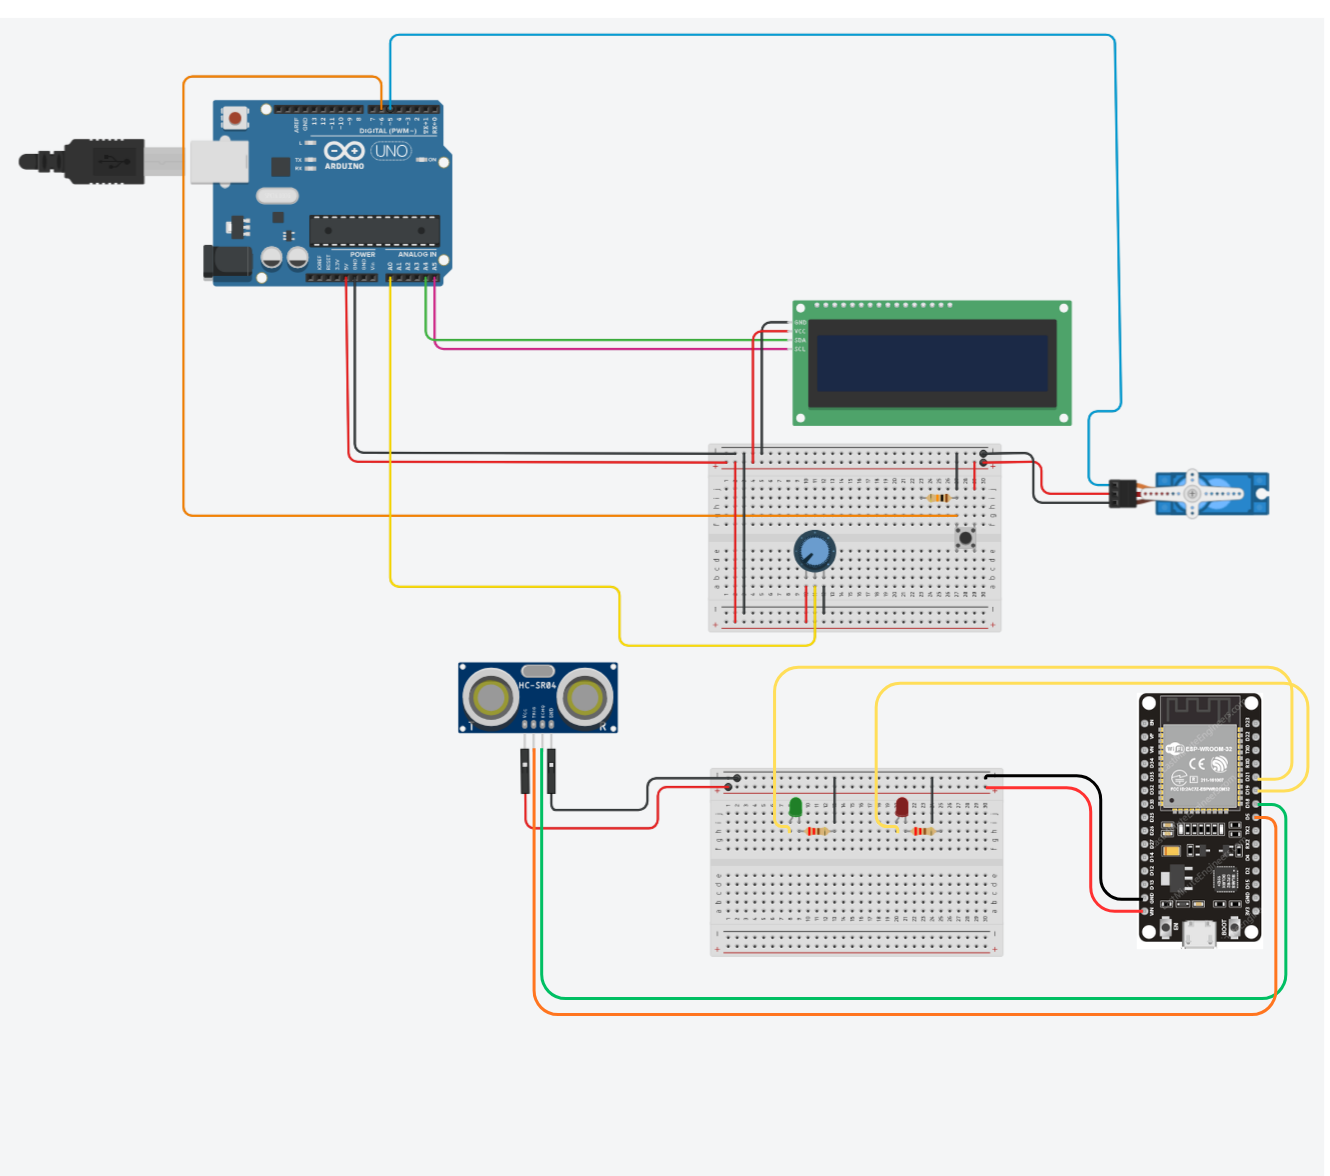
\includegraphics[width=0.85\textwidth]{tinkercad.png}
    \caption{Rappresentazione della breadboard e schema circuitale (TMS e WCS).}
    \label{fig:schema_hw}
\end{figure}

\subsection{Componenti e Pin Mapping -- TMS (ESP32)}

\begin{itemize}
    \item \textbf{Sonar HC-SR04 -- \texttt{Trig: Pin 5, Echo: Pin 18}:} Misura il livello dell'acqua nel serbatoio tramite impulsi ultrasonici. Il valore di distanza viene periodicamente campionato e inviato al CUS via MQTT.
    \item \textbf{LED Verde -- \texttt{Pin 17}:} Acceso quando la connessione Wi-Fi e MQTT è operativa e l'invio dei dati avviene correttamente.
    \item \textbf{LED Rosso -- \texttt{Pin 19}:} Acceso in caso di problemi di rete (Wi-Fi o MQTT non disponibili), segnalando all'operatore locale uno stato di errore.
\end{itemize}

\subsection{Componenti e Pin Mapping -- WCS (Arduino UNO)}

\begin{itemize}
    \item \textbf{Servomotore (valvola) -- \texttt{Pin 10}:} Controlla l'apertura del canale idraulico. L'intervallo operativo va da $0°$ (valvola chiusa, 0\% apertura) a $90°$ (valvola completamente aperta, 100\% apertura). Utilizza la libreria \texttt{ServoTimer2} per evitare conflitti con \texttt{TimerOne}.
    \item \textbf{Potenziometro B103 -- \texttt{Pin A0}:} Permette il controllo manuale dell'apertura della valvola in modalità \texttt{MANUAL}. Il valore analogico letto viene normalizzato nell'intervallo $[0.0, 1.0]$, con mapping invertito ($0\% \rightarrow 90°$, $100\% \rightarrow 0°$) per rispettare la meccanica del sistema. La sua posizione fisica è indipendente dal valore impostato da remoto tramite la dashboard. Questa limitazione hardware ha reso necessario implementare un meccanismo di \textit{pick-up} per la sincronizzazione tra controllo remoto e controllo locale (si veda la Sezione~\ref{sec:pickup}).
    \item \textbf{Pulsante Tactile -- \texttt{Pin 8}:} Commuta tra le modalità \texttt{AUTOMATIC} e \texttt{MANUAL}. Alla prima pressione si entra in \texttt{MANUAL}; alla seconda si torna in \texttt{AUTOMATIC}.
    \item \textbf{Display LCD I2C (16x2) -- \texttt{Indirizzo 0x27}:} Mostra il livello attuale di apertura della valvola in percentuale e la modalità operativa corrente (\texttt{AUTOMATIC}, \texttt{MANUAL} o \texttt{UNCONNECTED}).
\end{itemize}

% ─────────────────────────────────────────────
\section{Architettura Software}

\subsection{Struttura Generale del Sistema}

Tutti i sottosistemi embedded (TMS ed WCS) condividono lo stesso pattern architetturale: uno scheduler cooperativo basato su interrupt hardware (libreria \texttt{TimerOne}) con periodo base di \textbf{50ms}, task periodici definiti come sottoclassi di \texttt{Task}, e un oggetto \texttt{Context} come repository condiviso dello stato tra i task. Il backend Java è basato su \textbf{Vert.x} con architettura event-driven e comunicazione asincrona non bloccante.


% ─────────────────────────────────────────────
\section{TMS -- Tank Monitoring Subsystem (ESP32)}

\subsection{Task Concorrenti}

Il TMS è strutturato in tre task cooperativi gestiti dallo scheduler:

\begin{itemize}
    \item \textbf{SensorTask (periodo: 200ms):} Campiona il sonar HC-SR04 applicando una compensazione della temperatura per aumentare la precisione della misura. Il valore letto viene salvato nel \texttt{Context} condiviso, rendendolo disponibile al \texttt{PublishTask}.

    \item \textbf{PublishTask (periodo: 2000ms):} Legge il livello del serbatoio dal \texttt{Context} e lo pubblica sul broker MQTT. Aggiorna il LED verde o rosso in base all'esito della pubblicazione.

    \item \textbf{ConnectionTask (periodo: 1000ms):} Implementa una FSM a tre stati per la gestione della connettività. Si occupa di rilevare e recuperare automaticamente la perdita della connessione Wi-Fi o MQTT.
\end{itemize}

\subsection{FSM di Connettività (ConnectionTask)}

La macchina a stati gestisce tre stati distinti:

\begin{itemize}
    \item \texttt{CHECKING}: stato nominale. Verifica periodicamente che la connessione Wi-Fi e MQTT sia attiva. Se viene rilevata una disconnessione, transita nel rispettivo stato di riconnessione.
    \item \texttt{RECONNECTING\_WIFI}: tenta il ripristino della connessione Wi-Fi. Al successo, transita verso \texttt{RECONNECTING\_MQTT}.
    \item \texttt{RECONNECTING\_MQTT}: tenta la riconnessione al broker MQTT. Al successo, ritorna in \texttt{CHECKING}.
\end{itemize}

Le azioni di \textit{entry} in ogni stato sono gestite tramite il pattern \texttt{justEntered} + \texttt{checkAndSetJustEntered()}, che garantisce l'esecuzione unica delle operazioni di inizializzazione alla prima iterazione del task nello stato.

\subsection{Astrazione Hardware}

I device fisici sono nascosti dietro interfacce astratte (\texttt{ProximitySensor}, \texttt{Light}), con implementazioni concrete (\texttt{Sonar}, \texttt{Led}). La classe \texttt{TankMonitoringPlatform} funge da \textit{facade} per l'inizializzazione e l'accesso centralizzato all'hardware.

% ─────────────────────────────────────────────
\section{WCS -- Water Channel Subsystem (Arduino)}

\subsection{Task Concorrenti}

Il WCS è strutturato in tre task cooperativi:

\begin{itemize}
    \item \textbf{FSMController (periodo: 75ms):} Task principale che implementa la FSM dell'intero sottosistema. Gestisce le transizioni tra le modalità operative, aggiorna la valvola e il display LCD, e reagisce agli input del pulsante e ai comandi seriali.

    \item \textbf{PotReader (periodo: 200ms):} Campiona il valore del potenziometro e lo normalizza nell'intervallo $[0.0, 1.0]$, salvandolo nel \texttt{Context}. Attivo solo quando la FSM si trova in modalità \texttt{MANUAL}.

    \item \textbf{SerialTask (periodo: 50ms):} Gestisce la comunicazione bidirezionale con il CUS tramite porta seriale a 115200 baud. Riceve comandi di modalità e percentuale di apertura valvola, e trasmette lo stato corrente del WCS.
\end{itemize}

\subsection{FSM del Water Channel (FSMController)}

La macchina a stati gestisce tre stati operativi:

\begin{itemize}
    \item \texttt{AUTOMATIC}: la valvola è controllata interamente dal CUS tramite comandi seriali. Il display mostra la percentuale di apertura corrente e la dicitura \texttt{AUTOMATIC}. La pressione del pulsante provoca la transizione in \texttt{MANUAL}.

    \item \texttt{MANUAL}: l'operatore locale controlla direttamente la valvola tramite il potenziometro. Il display mostra la percentuale corrente e la dicitura \texttt{MANUAL}. La pressione del pulsante riporta alla modalità \texttt{AUTOMATIC}. In questo stato, il WCS notifica al CUS la modalità attiva per sincronizzare il sistema distribuito.

    \item \texttt{UNCONNECTED}: il CUS non è raggiungibile (timeout seriale). Il display mostra \texttt{UNCONNECTED}. Il sistema mantiene l'ultima posizione nota della valvola fino al ripristino della connessione.
\end{itemize}

\textbf{Soglie di controllo automatico (CUS → WCS):}
\begin{itemize}
    \item Livello $> L_1$ (20\%) per più di $T_1$ secondi $\rightarrow$ valvola al \textbf{50\%}.
    \item Livello $> L_2$ (40\%) $\rightarrow$ valvola al \textbf{100\%} immediatamente.
    \item Livello rientrato sotto la soglia $\rightarrow$ valvola richiusa.
\end{itemize}

\subsection{Comunicazione Seriale Asincrona -- MsgService}

La comunicazione con il CUS avviene in modo non bloccante tramite la classe \texttt{MsgService}. I caratteri in arrivo vengono accumulati in un buffer; quando viene rilevato il terminatore \texttt{\textbackslash n}, la stringa è impacchettata in un oggetto \texttt{Msg} e un flag \texttt{msgAvailable} viene alzato. Il \texttt{SerialTask} verifica il flag ad ogni ciclo e processa il messaggio senza mai bloccarsi in attesa. Il protocollo è basato su messaggi ASCII distinti, terminati da \texttt{\textbackslash n}:

\begin{itemize}
    \item \texttt{MODE:\{MODE\}} -- inviato dal CUS al WCS per imporre la modalità operativa (es.\ \texttt{MODE:AUTOMATIC}), oppure dal WCS al CUS per notificare un cambio di modalità indotto localmente (es.\ \texttt{MODE:MANUAL} in seguito alla pressione del pulsante).
    \item \texttt{VALVE:\{PERCENT\}} -- inviato dal CUS al WCS per impostare la percentuale di apertura target della valvola (es.\ \texttt{VALVE:50}); il WCS può a sua volta inviare la percentuale corrente al CUS per la sincronizzazione dello stato.
\end{itemize}

\subsection{Meccanismo di Pick-Up -- Sincronizzazione Potenziometro e Dashboard}
\label{sec:pickup}

In modalità \texttt{MANUAL} il controllo della valvola può provenire da due sorgenti distinte: il potenziometro fisico sul WCS e lo slider della dashboard remota (DBS). Il potenziometro adottato è un componente passivo a rotazione limitata: non è motorizzato né di tipo \textit{endless}, il che rende impossibile aggiornarne la posizione meccanica a seguito di un comando remoto. Se lo slider della DBS impostasse direttamente la posizione del motore, il valore del potenziometro e quello visualizzato sul display risulterebbero immediatamente sfasati, causando un \textit{reset} incontrollato della valvola non appena l'operatore ruotasse fisicamente la manopola.

\textbf{Soluzione -- meccanismo di pick-up:} quando il WCS riceve un comando \texttt{VALVE:XX} dal CUS in modalità \texttt{MANUAL}, il motore \emph{non} viene mosso immediatamente. Il valore target viene invece memorizzato nel \texttt{Context} (\texttt{targetValveFromDBS}) e viene attivato un flag \texttt{dbsControlActive}. Ad ogni tick, il \texttt{PotReader} confronta la lettura corrente del potenziometro con il target: non appena la differenza scende al di sotto della soglia \texttt{PICKUP\_THRESHOLD} (2\%), il flag viene abbassato, il motore si porta alla posizione del potenziometro e il WCS notifica il nuovo valore al CUS tramite \texttt{VALVE:XX}. Da quel momento il potenziometro torna ad avere il controllo diretto della valvola.

La soglia del 2\% è stata scelta come compromesso tra la precisione necessaria per un aggancio pulito e la tolleranza al rumore analogico del sensore, che rende impraticabile una soglia inferiore all'1\%.

\textbf{Gestione dello stato UNCONNECTED in modalità MANUAL:} una criticità correlata riguarda il comportamento del CUS quando il TMS smette di trasmettere dati. Nella logica originale, il timeout MQTT avrebbe fatto transitare il sistema in \texttt{UNCONNECTED} anche durante una sessione di controllo manuale, disabilitando lo slider sulla dashboard. La correzione applicata nel \texttt{DataService} del CUS vincola la transizione in \texttt{UNCONNECTED} alla sola modalità \texttt{AUTOMATIC}: in \texttt{MANUAL} il sistema rimane operativo indipendentemente dalla connettività del TMS, poiché la policy automatica è comunque sospesa.

% ─────────────────────────────────────────────
\section{CUS -- Control Unit Subsystem (Java/Vert.x)}

\subsection{Framework e Architettura}

Il backend è sviluppato con \textbf{Vert.x 4.2.6}, un framework event-driven e non bloccante per la JVM. Vert.x permette di gestire simultaneamente le tre interfacce di comunicazione del CUS (MQTT, seriale, HTTP) senza ricorrere a thread multipli bloccanti, grazie al modello basato su \textit{Verticle} e \textit{Event Bus}.

\subsection{Protocolli e Classi di Comunicazione}

\begin{itemize}
    \item \textbf{MQTTProtocol}: utilizza il client \textit{Eclipse Paho} in modalità callback. Sottoscrive il topic pubblicato dal TMS e aggiorna il timestamp dell'ultimo dato ricevuto per rilevare situazioni di \texttt{UNCONNECTED} (timeout $T_2$).

    \item \textbf{SerialProtocol}: utilizza la libreria \texttt{jssc} con un \texttt{SerialPortEventListener} per la ricezione asincrona dei dati dal WCS. Una \texttt{BlockingQueue} funge da buffer di decoupling tra il thread seriale e il loop Vert.x, garantendo thread-safety.

    \item \textbf{HTTPProtocol}: esposto tramite \texttt{Vert.x Web}, serve le API REST consumate dalla dashboard. Utilizza \texttt{Vert.x WebClient} per eventuali chiamate HTTP interne in modalità non bloccante con futures/callback.
\end{itemize}

\subsection{API REST (DataService Verticle)}

Il \texttt{DataService} espone i seguenti endpoint HTTP:

\begin{itemize}
    \item \texttt{GET /api/data} -- restituisce le ultime $N$ misurazioni del livello del serbatoio (buffer circolare in memoria, \texttt{LinkedList} con massimo 10 elementi).
    \item \texttt{GET /api/status} -- restituisce lo stato corrente del sistema: \texttt{AUTOMATIC}, \texttt{MANUAL} o \texttt{UNCONNECTED}.
    \item \texttt{POST /api/status} -- permette alla dashboard di commutare la modalità operativa del sistema (corpo JSON: \texttt{\{"mode": "MANUAL"\}}). Il CUS propaga il cambio al WCS tramite il messaggio seriale \texttt{MODE:\{MODE\}}.
    \item \texttt{GET /api/valve} -- restituisce la percentuale di apertura corrente della valvola.
    \item \texttt{POST /api/valve} -- permette alla dashboard di impostare la percentuale di apertura della valvola in modalità \texttt{MANUAL}. Il CUS inoltra il valore al WCS tramite il messaggio seriale \texttt{VALVE:\{PERCENT\}}.
\end{itemize}

\subsection{Logica di Controllo Automatico}

Il \texttt{CUS} implementa la policy di controllo del livello secondo le seguenti regole:

\begin{enumerate}
    \item Se il livello supera $L_1$ per più di $T_1$ secondi, il CUS invia al WCS il comando di aprire la valvola al 50\%. La valvola viene richiusa quando il livello scende sotto $L_1$.
    \item Se il livello supera $L_2$ (indipendentemente dal tempo), la valvola viene aperta al 100\% immediatamente. Viene richiusa quando il livello scende sotto $L_2$.
    \item Se non vengono ricevuti dati dal TMS per più di $T_2$ secondi, il sistema transita nello stato \texttt{UNCONNECTED}, sospendendo le operazioni automatiche. Il ripristino avviene non appena i dati tornano disponibili.
\end{enumerate}

\subsection{Design Pattern Adottati}

\begin{itemize}
    \item \textbf{Callback/Listener}: per operazioni asincrone su MQTT e seriale.
    \item \textbf{Observer}: per la propagazione degli eventi di cambio modalità (\texttt{ModeChangeCallback}) e cambio valvola (\texttt{ValveChangeCallback}).
    \item \textbf{Message Queue} (\texttt{BlockingQueue}): per il disaccoppiamento tra il thread seriale di \texttt{jssc} e il thread principale Vert.x.
    \item \textbf{Protocol Adapter}: ciascun protocollo (MQTT, seriale, HTTP) è incapsulato in una classe dedicata che adatta le chiamate native all'interfaccia del CUS.
    \item \textbf{Façade} (\texttt{CUSService}): centralizza l'orchestrazione dei tre protocolli, nascondendo la complessità interna.
\end{itemize}

% ─────────────────────────────────────────────
\section{DBS -- Dashboard Subsystem (Web)}

La dashboard è implementata come \textbf{applicazione web statica} (HTML + CSS + JavaScript puro), senza dipendenze da framework pesanti. Effettua polling verso le API del CUS ogni secondo.

\subsection{Visualizzazione}

\begin{itemize}
    \item \textbf{Grafico livello serbatoio}: realizzato con la libreria \texttt{Chart.js}, mostra le ultime $N$ misurazioni ricevute dal CUS in forma di grafico a linea aggiornato in tempo reale.
    \item \textbf{Percentuale apertura valvola}: indicatore numerico e/o barra di progressione che riflette lo stato attuale della valvola.
    \item \textbf{Stato del sistema}: badge testuale colorato che mostra \texttt{AUTOMATIC}, \texttt{MANUAL}, \texttt{UNCONNECTED} o \texttt{NOT AVAILABLE} (quest'ultimo quando il CUS non è raggiungibile).
\end{itemize}

\subsection{Controllo}

\begin{itemize}
    \item \textbf{Pulsante modalità}: commuta tra \texttt{AUTOMATIC} e \texttt{MANUAL} inviando una richiesta \texttt{POST /api/status} al CUS. Il backend, ricevuta la richiesta, propaga il cambio di modalità al WCS tramite il messaggio seriale \texttt{MODE:\{MODE\}}.
    \item \textbf{Slider valvola}: visibile e attivo solo in modalità \texttt{MANUAL}. Permette di impostare la percentuale di apertura desiderata inviando una richiesta \texttt{POST /api/valve} al CUS, il quale inoltra il comando al WCS tramite il messaggio seriale \texttt{VALVE:\{PERCENT\}}. A seguito del comando, lo slider rimane fisso sul valore impostato fino a quando il potenziometro fisico non raggiunge quella posizione e ne acquisisce il controllo tramite il meccanismo di pick-up; solo allora il valore visualizzato torna ad aggiornarsi in base alle letture del potenziometro.
\end{itemize}

% ─────────────────────────────────────────────
\section{Pattern Comuni ai Sottosistemi Embedded}

I sottosistemi TMS (ESP32) e WCS (Arduino) condividono un'identica architettura interna, che garantisce coerenza, riutilizzabilità e facilità di manutenzione:

\begin{enumerate}
    \item \textbf{Cooperative Task Scheduler}: scheduler basato su interrupt \texttt{TimerOne} con periodo base di 50ms. Ogni task dichiara il proprio periodo e viene invocato esclusivamente quando il suo intervallo è scaduto. Nessun task è bloccante.

    \item \textbf{FSM Enum-Based}: le macchine a stati sono implementate tramite \texttt{enum} C++ e blocchi \texttt{switch/case}, senza overhead di ereditarietà. Le azioni di entry vengono eseguite una sola volta grazie al pattern \texttt{justEntered}.

    \item \textbf{Context / Shared State}: un unico oggetto \texttt{Context} per sottosistema funge da repository condiviso. I task non comunicano mai direttamente tra loro: scrivono e leggono esclusivamente tramite il \texttt{Context}, eliminando ogni accoppiamento diretto.

    \item \textbf{Façade Pattern} (\texttt{Platform}): le classi \texttt{TankMonitoringPlatform} e \texttt{WaterChannelPlatform} centralizzano l'inizializzazione e l'accesso all'hardware, nascondendo i dettagli di configurazione dei pin.

    \item \textbf{Interface Segregation}: ogni device fisico è rappresentato da un'interfaccia astratta (\texttt{Light}, \texttt{ProximitySensor}, \texttt{Button}) con una o più implementazioni concrete. Questo permette di sostituire o simulare i componenti hardware senza modificare la logica dei task.

    \item \textbf{Message Passing Asincrono}: la comunicazione con il backend avviene tramite \texttt{MsgService}, che garantisce ricezione non bloccante via buffer e flag di disponibilità.
\end{enumerate}

% ─────────────────────────────────────────────
\section{Difficoltà Riscontrate e Conclusioni}

\subsection{Difficoltà Riscontrate}

\begin{itemize}
    \item \textbf{Sincronizzazione potenziometro fisso e slider remoto:} L'utilizzo di un potenziometro passivo a rotazione limitata ha impedito di adottare un controllo diretto della posizione dalla dashboard: muovere immediatamente il motore al valore remoto avrebbe causato un disallineamento persistente tra la manopola fisica e lo stato visualizzato, con successive sovrascritture indesiderate alla prima rotazione del potenziometro. Il problema è stato risolto con il meccanismo di pick-up descritto nella Sezione~\ref{sec:pickup}, che ritarda il trasferimento del controllo al potenziometro fino a quando questo non raggiunge fisicamente il valore target impostato da remoto. Il potenziomentro viene preso come single source of truth inizalmente e sovrascritto dal controllo remoto neccessitando il pick in per riacquisire il controllo (questo evita discrepanze tra WCS e DBS).

    \item \textbf{Conflitti tra librerie Timer su Arduino:} L'utilizzo simultaneo di \texttt{TimerOne} (per lo scheduler) e della libreria standard \texttt{Servo} ha generato conflitti sui timer hardware dell'ATmega328P. Il problema è stato risolto adottando \texttt{ServoTimer2}, che utilizza \texttt{Timer2} lasciando \texttt{Timer1} libero per lo scheduler.

    \item \textbf{Sincronizzazione thread seriale e Vert.x:} La libreria \texttt{jssc} esegue i callback di ricezione seriale in un thread separato rispetto al loop Vert.x. Questo ha reso necessario l'uso di una \texttt{BlockingQueue} per il passaggio sicuro dei messaggi tra i due contesti di esecuzione, evitando race condition.

    \item \textbf{Gestione dello stato UNCONNECTED distribuito:} Coordinare la transizione in \texttt{UNCONNECTED} in modo coerente tra CUS (timeout MQTT), WCS (timeout seriale) e DBS (CUS non raggiungibile) ha richiesto un'attenta definizione dei timeout e dei meccanismi di ripristino per ciascun sottosistema.

    \item \textbf{Latenza del polling dashboard:} Il polling HTTP ogni secondo introduce una latenza percettibile nella visualizzazione degli aggiornamenti. Per un sistema di produzione si valuterebbe l'adozione di WebSocket o Server-Sent Events per aggiornamenti in push.
\end{itemize}

\subsection{Conclusioni}

Lo sviluppo dello \textit{Smart Tank Monitoring System} ha dimostrato come un'architettura distribuita e modulare -- basata su task cooperativi, FSM leggere e design pattern consolidati -- permetta di realizzare un sistema IoT reattivo e manutenibile anche con risorse hardware limitate.

La separazione netta delle responsabilità tra i quattro sottosistemi ha semplificato lo sviluppo parallelo e il debugging: ciascun componente poteva essere testato indipendentemente prima dell'integrazione finale. I pattern comuni condivisi tra TMS e WCS hanno ridotto significativamente la duplicazione del codice e reso immediata la comprensione di entrambi i firmware.

Il sistema finale rispetta i requisiti funzionali: monitoraggio continuo del livello, controllo automatico e manuale della valvola, rilevamento di perdita di connettività e dashboard web in tempo reale.


\section{Link al video dimostrativo}
Il video dimostrativo del sistema in azione è disponibile al seguente link: \href{https://liveunibo-my.sharepoint.com/:v:/g/personal/giuseppe_cattolico_studio_unibo_it/IQBa6F1gB55XSLYPmsERKnfZAb7FWOWHKEoVaHiGJA5QiC4?nav=eyJyZWZlcnJhbEluZm8iOnsicmVmZXJyYWxBcHAiOiJPbmVEcml2ZUZvckJ1c2luZXNzIiwicmVmZXJyYWxBcHBQbGF0Zm9ybSI6IldlYiIsInJlZmVycmFsTW9kZSI6InZpZXciLCJyZWZlcnJhbFZpZXciOiJNeUZpbGVzTGlua0NvcHkifX0&e=65CfIX}{Clicca qui }
\end{document}